\chapter{Visione artificiale}
\label{chap:visione}

\begin{minipage}{12cm}\textit{In questo capitolo verrà trattato il problema della generazione dei set di coppie di punti omologhi usando tecniche di visione. In particolare si utilizzeranno tecniche di Feature Detection e stereoscopia.}
\end{minipage}

\vspace*{1cm}

Nel capitolo \ref{chap:visualObs} si è accennato agli strumenti che sarebbero stati usati al fine della generazione dei suddetti set. In questo capitolo si procederà ad illustrarne il funzionamento con maggior dettaglio e si fornirà una possibile soluzione al problema. Conviene definire per primo il problema che si vuole affrontare.

\begin{prob}
	\label{prob:vis:gensets}
	Sia un osservatore mobile dotato di almeno due fotocamere. Si supponga ancora capace di "catturare", attraverso le suddette fotocamere, coppie di foto in diversi istanti (anche regolari). Allora: 
	\begin{enumerate}
		\item è possibile, utilizzando le informazioni fornite dalle fotocamere, calcolare le coordinate spaziali (in $\mathbb{R}^3$) di un punto del mondo (o più di uno) nel sistema di riferimento solidale all'osservatore?
		\item dato un punto del mondo (o più di uno) per il quale si è riusciti a calcolarne le coordinate spaziali, è possibile individuare lo stesso punto, in un altro istante del tempo, se l'osservatore si è mosso e se lo stesso è ancora visibile?  
	\end{enumerate}
\end{prob}

\section{Feature Detection e Matching}
\label{sec:feature}
Per \textbf{Feature Detection} o \textbf{individuazione dei punti chiave} in italiano, si intende un particolare settore facente parte della branca della visione artificiale, il cui scopo è quello di per l'appunto l'individuazione, la descrizione e il confronto delle Feature. Ma che cosa è una Feature?
In generale risulta difficile fornire una definizione chiara di cosa è una \textbf{Feature} o \textbf{Punto chiave}, può dipendere ad esempio dall'algoritmo che si utilizza o da scelte implementative.


\begin{figure}[h]
	\centering
	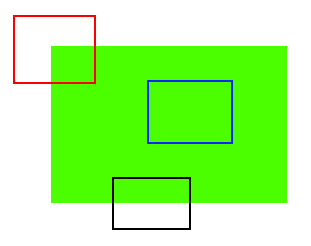
\includegraphics[width=420pt]{imgs/feature_simple.png}
	\caption{Individuazione delle Features.}
	\label{vis:feature:detect}
\end{figure} 

Si faccia ad esempio riferimento alla figura \ref{vis:feature:detect}, si supponga di dover individuare una buon punto chiave, il quale possa essere facilmente riconosciuto e riposizionato. Si consideri per prima la porzione di immagine evidenziata dal riquadro blu; è chiaro che qualora si dovesse scegliere dove posizionare tale blocco, si avrebbero un numero elevatissimo di possibilità ed in nessun caso si potrebbe avere al certezza di un buon posizionamento. Si consideri allora il blocco nero, in questo caso il numero delle possibilità è sicuramente inferiore, infatti esso può essere posizionato solo nel lato inferiore del rettangolo verde in figura. Infine si consideri il blocco rosso, è chiaro che quello in figura è l'unico punto in cui esso può essere posizionato.
L'esempio precedente fornisce un importantissimo spunto ri riflessione su cosa può essere una Feature e cosa no. Infatti sicuramente una porzione di immagine uniforme non può essere un punto chiave; se invece si considerano dei contorni di un oggetto la situazione migliora. In particolare se si considera il contorno di un oggetto e se ne sceglie un punto che abbia una forma o pattern particolare, come ad esempio uno spigolo di un oggetto, risulta molto più facile un eventuale riconoscimento. 

Ovviamente l'esempio precedente risulta estremizzato. Infatti, in un caso reale, le Feature possono essere ruotate e/o scalate e questo complica il problema. Al contempo però, il mondo reale risulta più dettagliato e risulta più difficile avere uno stesso pattern in punti diversi.

Si è fornita, quanto meno in modo informale, una definizione di Feature. Nei prossimi paragrafi con ordine si illustreranno tre algoritmi: il primo adibito all'individuazione delle features, il secondo viene impiegato per la generazione dei descrittori (che come si vedrà sono utilizzati per distinguere i punti chiave in base alle informazioni fornite dall'immagine) ed il terzo è un matcher. 

%\subsection{Definizioni e problema}
%\label{sec:det:def}
\subsection{L'algoritmo FAST}
\label{sec:det:fast}
L'algoritmo FAST (Feature from Accelerated Segment Test) è un algoritmo adibito all'estrazione dei punti chiave da un immagine, sviluppato originariamente da Edward Rosten e Tom Drummond nel 2006 \cite{bib2}. Esistono numerosi algoritmi adibiti a questo scopo, ed alcuni riescono anche ad ottenere risultati più accurati. In accordo con il nome dell'algoritmo però quest'ultimo risulta particolarmente veloce e in generale fornisce risultati molto buoni. In accordo con le specifiche di esecuzione realtime già accennate, pertanto la scelta è ricaduta su quest'ultimo. Inoltre l'algoritmo FAST è privo di licenze a pagamento e può essere liberamente impiegato in progetti sia di ricerca che commerciali. Di seguito se ne illustra il funzionamento.
\newline \newline
Si consideri un pixel $p$, sia $I_p$ la sua intensità e siano fissate una soglia di funzionamento $t$ e un intero $n$. Si vuole verificare se il pixel $p$ può essere considerato una Feature oppure no. 

\begin{figure}[h]
	\centering
	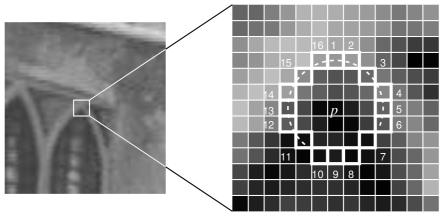
\includegraphics[width=420pt]{imgs/fast_speedtest.jpg}
	\caption{Fast Segment test.}
	\label{vis:feature:Fast}
\end{figure} 
  
 
In accordo con quanto detto nel precedente paragrafo, uno spigolo/angolo può essere considerato una buon punto chiave. Il \textbf{test} ricerca questo tipo di punti e viene effettuato nel modo seguente:
\begin{enumerate}
	\item Si consideri un cerchio di 16 pixel intorno a $p$, evidenziato in figura \ref{vis:feature:detect} dai pixel riquadrati.
	\item Il punto $p$ è uno spigolo se vale che un numero $n$ di pixel appartenenti al suddetto cerchio hanno intensità o tutti maggiore di $I_p + t$ o tutti minore di $I_p - t$.
\end{enumerate}

Osservando sempre la figura \ref{vis:feature:detect} si intuisce la motivazione del test. Infatti uno spigolo, indipendentemente da come è ruotato, avrà una forma convessa. Si intuisce che la buona riuscita del test dipende dalla scelta dei parametri $t, n$, tipicamente si sceglie $n = 12$, $t$ dipende dal tipo di immagini utilizzate.

	Nella pratica si inserisce un \textbf{test veloce} per effettuare una prima scrematura dei punti. Con riferimento alla figura \ref{vis:feature:detect} si controllano solo i pixel 1, 9, 5 e 13. Si verifica se i pixel 1 e 9 hanno una differenza assoluta di intensità rispetto a $p$ maggiore della soglia $t$, in caso si analizzano anche i pixel 5 e 13. Se $p$ è uno spigolo deve valere allora che 3 di tali pixel devono essere più intensi di $p$ e uno meno intenso, dove l'intensità e verificata con al soglia $t$ ovviamente.

Si può notare che se la condizione del test veloce non è verificata allora non c'è modo che il test completo possa avere un buon esito, perché non possono esistere n pixel contigui più intensi o meno intensi di $p$. In generale dei falsi positivi possono superare il test veloce e quindi il testo completo deve essere impiegato per ottenere un risultato corretto.

L'algoritmo allo stato attuale però presenta alcune criticità:
\begin{enumerate}
	\item Per $n < 12$ il test veloce non può essere generalizzato perché un pixel $p$ può superare il test completo anche se solo due dei pixel selezionati sono meno intensi e due più intensi.
	\item L'efficienza del test dipende dalla scelta e dall'ordinamento dei pixel selezionati per il test. In genere però i punti cui il successo del test dipende da questi fattori non sono buone feature. 
	\item Molte feature vengono individuate una adiacente all'altra.
\end{enumerate} 

Per risolvere il terzo problema si introduce un ulteriore passo detto \textbf{non-maximal suppression}:
\begin{enumerate}
	\item Si calcola una funzione valore $V$ per tutti i punti chiave individuati. La funzione $V$ per il punto chiave $p$ è pari alla somma della differenza assoluta tra l'intensità di $p$ e i 16 pixel considerati intorno allo stesso durante il test.
	\item Se i punti chiave $p_1$ e $p_2$ sono adiacenti, ovvero hanno una distanza in pixel minore di una soglia $d$, si scarta quello che ha la funzione valore più bassa.
\end{enumerate}
Il precedente test è pensato in modo che, in caso di necessità, vengono scartati i punti chiave meno "marcati" e conseguentemente meno distinguibili. 

L'ultimo passo che può essere impiegato per aumentare le prestazioni del rilevatore FAST è quello di impiegare una \textbf{rete neurale}. Essa può essere addestrata utilizzando i risultati forniti dello stesso FAST al fine di sostituire e combinare il test veloce e quello completo. A patto che il set di addestramento sia abbastanza vario e comprensivo di rumore, un addestramento supervisionato può ottenere un buon grado di efficacia ed efficienza. 
% scrivere sta roba%

In figura \ref{vis:feature:detection} è possibile ammirare un esempio di individuazione dei punti chiave in un immagine. Quest'ultimi sono indicati con dei cerchi colorati. Inoltre si è utilizzata la soppressione dei punti chiave troppo vicini, utilizzando il concetto di non-maximal suppression.
\begin{figure}[h]
	\centering
	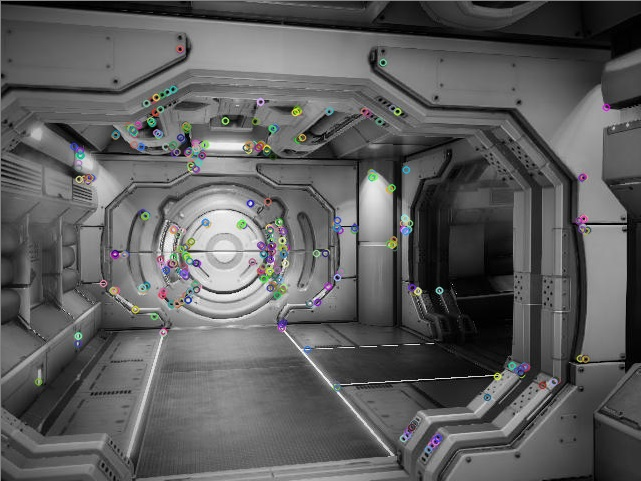
\includegraphics[width=420pt]{imgs/fdetection.jpg}
	\caption{Risultato dell'esecuzione dell'algoritmo FAST con non-maximal suppression attivata.}
	\label{vis:feature:detection}
\end{figure} 

Si conclude la presentazione dell'algoritmo con alcune riflessioni. FAST è un algoritmo di tipo euristico, come molti altri, ma nel caso generale risulta molto efficace. Per quanto riguarda il test in essere esso ha un basso impatto computazionale, inoltre il test può essere eseguito in parallelo per molti pixel alla volta. Esso si presta ad una facile e efficiente implementazione sia su CPU (sfruttando la vettorizzazione) sia su GPU.

\subsection{L'algoritmo BRIEF}
\label{sec:det:brief}
Nel precedente paragrafo si è introdotto il concetto di punto chiave e si è fornito un algoritmo atto al loro calcolo. Per poter procedere però, è necessario un ulteriore strumento atto a confrontarli. Infatti essi sono semplicemente delle coordinate in pixel. Occorre perciò definire un confronto tra punti chiave.

Si introduce il concetto di \textbf{descrittori}. Anche in questo caso una definizione formale è difficile da fornire. Infatti, la forma e il funzionamento del descrittore è fortemente dipendente dall'algoritmo scelto. Informalmente, potremmo definire un descrittore come "un'impronta" o una "firma" del punto chiave. Un descrittore è considerato efficace se presenta la caratteristica di associare una firma molto differente a punti chiave simili.

In letteratura esistono differenti tipologie di descrittori e algoritmi atti al loro calcolo; alcuni ad esempio utilizzando come firma dei valori in virgola mobile, altri utilizzano delle stringhe di bit. Essi si differenziano inoltre per il carico computazionale, di memoria e naturalmente per efficacia.
Considerando l'obbiettivo real-time di questo lavoro di tesi, la scelta dell'algoritmo da utilizzare è ricaduta sull'algoritmo BRIEF. Esso infatti risulta veloce, ha poco impatto sulla memoria, e nel caso generale ha efficacia paragonabile ai suoi contendenti.

L'algoritmo BRIEF, Binary Robust Independent Elementary Features, è presentato in \cite{bib4}. Esso genera dei descrittori sotto forma di stringhe di bit. Il vantaggio principale di considerare stringhe è che il confronto tra due keypoint può essere fatto in modo estremamente efficiente, con una sola operazione XOR.

L'algoritmo BRIEF, durante il calcolo dei descrittori, fa inoltre in modo di mappare keypoint molto vicini in descrittori molto distanti, dove la distanza per le stringhe descrittrici può essere calcolata come la distanza di Hamming.

In genere, algoritmi di tipo stringa, per ottenere i descrittori utilizzano tecniche simili ad HASH, talvolta rinforzate. In particolare, BRIEF funziona in questo modo:
\begin{enumerate}
	\item Si fissa un pattern di confronto, cioè viene fissato quali dei pixel appartenenti ad un intorno del punto chiave saranno utilizzati nel calcolo. Si selezionano, quindi, $n_d$ pixel, dove $n_d$ è la lunghezza in bit del descrittore. Esempi di pattern possono essere:
	\begin{enumerate}
		\item uniforme: i pixel scelti sono distribuiti in maniera uniforme dentro un quadrato centrato nel punto chiave. 
		\item gaussiano: si utilizza una pseudo-distribuzione gaussiana, cioè si prendono più pixel vicino al punto chiave.
		\item randomico: i pixel sono scelti a caso all'interno del suddetto quadrato.
	\end{enumerate}
	\item Per evitare che a causa di disturbo nell'immagine per uno stesso punto chiave si possano avere differenti descrittori, si applica un pre filtraggio dell'immagine stessa.
	\item Per ogni bit della stringa ed in base al pattern scelto se ne fissa il valore secondo la formula:
	\begin{equation}
		\tau_i(p, q_i) := \begin{cases}
		1, \qquad se \; I_p \leq I_{q_i}\\
		0, \qquad altrimenti
		\end{cases}
	\end{equation}
	dove con $p$ si è indicato il pixel punto chiave, $q_i$ l'i-esimo pixel scelto in base al pattern, appartente ad un intorno di $p$. Per $I_p$, come per il paragrafo precedente, si intende l'intensità del pixel $p$.
\end{enumerate}

In \cite{bib4} si può trovare una descrizione più accurata dei pattern, dei vari test di performance e confronti con altri algoritmi di descrizione. Si può evincere che a fronte di una maggiore velocità di esecuzione, si ha un efficienza identica o talvolta superiore ai suoi contendenti.

Da punto di vista implementativo, si fa notare che è altamente parallelizzabile sia su CPU vettorizzate sia su GPU.
\subsection{Brute Force matching}
\label{sec:det:bmmatch}

Fino a questo punto si è in grado di calcolare e descrivere i punti chiave di un immagine. Per assolvere il problema proposto si deve essere in grado di relazionare ciascun punto chiave di un immagine al suo corrispettivo in una seconda (ovviamente se esso è visibile nella seconda). 

Resta da definire allora un ultimo concetto, cioè la struttura del comparatore o matcher che dovrebbe essere usata. Le scelte fatte nei precedenti paragrafi, insieme ad una implementazione che vedremo sarà altamente parallela, semplificano moltissimo questo ultimo punto. Infatti si utilizza un \textbf{comparatore a forza bruta}. Ogni punto chiave individuato nella prima immagine lo si confronta con tutti quelli individuati nella seconda. Il confronto è fatto attraverso il calcolo della distanza di Hamming tra i descrittori. Si sceglie poi quello che ha dato luogo alla distanza di Hamming più piccola. Per escludere dei falsi positivi si fissa una soglia minima per il riconoscimento, questo evita che un punto chiave non presente nella seconda immagine possa essere associato ad un altro differente.

Sebbene possa sembrare non efficiente come approccio, si deve rammentare che una grande ottimizzazione è stata effettuata a monte grazie ai descrittori. Inoltre su architetture vettorizzate o su GPU un eventuale confronto più intelligente basato su percorsi decisionali darebbe luogo alla fine pratica ad un tempo di esecuzione solo maggiore. Infatti la regola base in questo tipo di architetture è che si devono evitare differenti percorsi logici tra i vari thread, pena perdita di parallelismo.

Si mostrano due esempi di esecuzione rispettivamente in figura \ref{vis:feature:risStereo} e \ref{vis:feature:risTwo}. Le immagini campione sono affiancate, con dei cerchi colorati si indicano i punti chiave e con dei segmenti colorati le associazioni trovate. Si noti come grazie alla soglia limite ai punti chiave poco marcati o quelli non presenti nella seconda foto non vengano associati punti chiave errati.
\begin{figure}[h!]
	\centering
	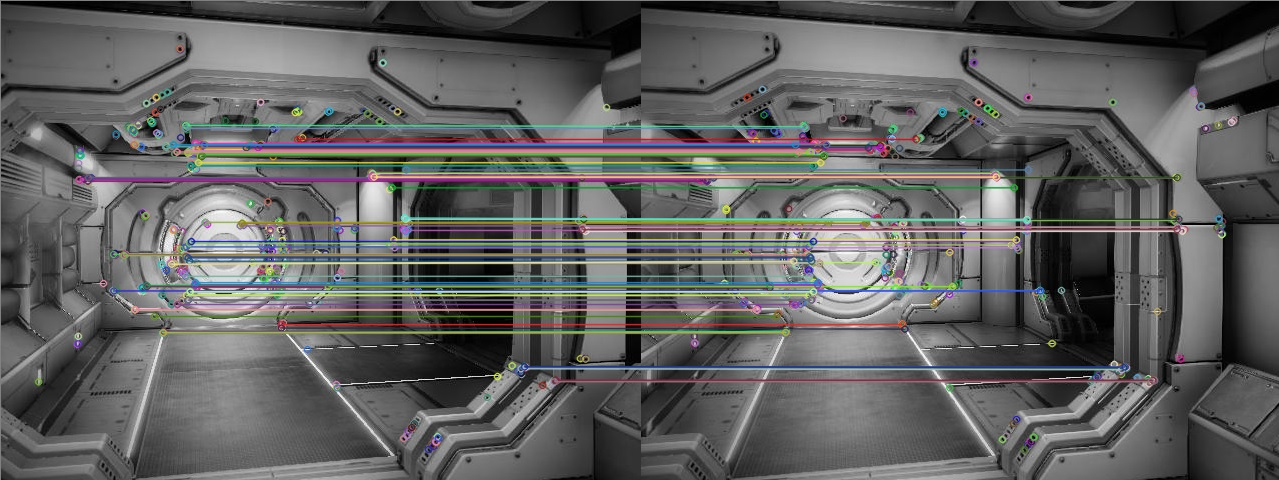
\includegraphics[width=420pt]{imgs/stereoDetection.jpg}
	\caption{Risultato dell'esecuzione del comparatore: FAST + BRIEF + Brute Force matcher su una coppia di immagini stereo.}
	\label{vis:feature:risStereo}
\end{figure} 

\begin{figure}[h!]
	\centering
	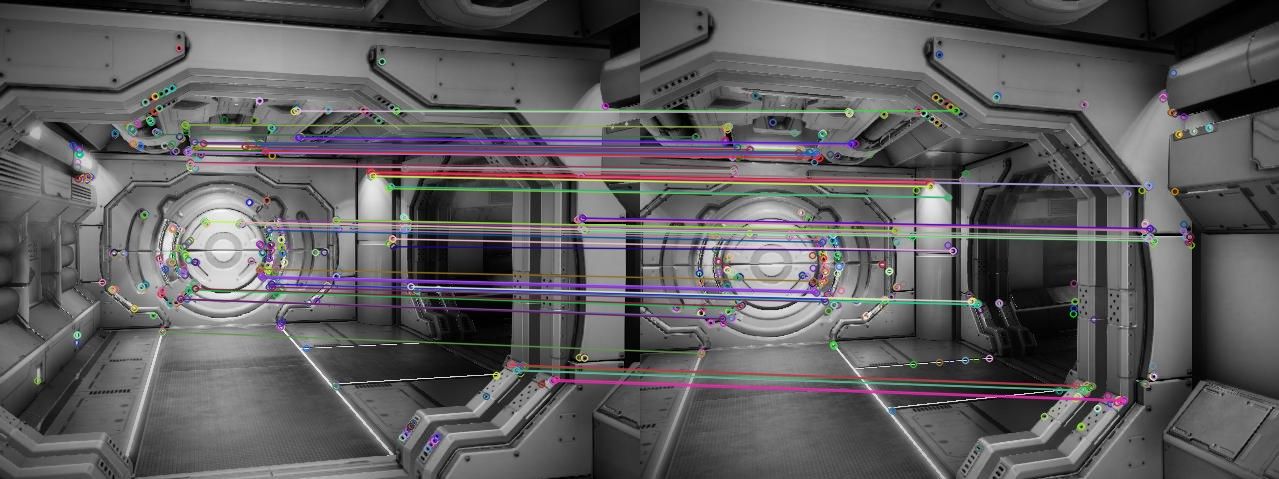
\includegraphics[width=420pt]{imgs/TwoInstantDetection.jpg}
	\caption{Risultato dell'esecuzione del comparatore: FAST + BRIEF + Brute Force matcher su due immagini in due punti di osservazione diversi}
	\label{vis:feature:risTwo}
\end{figure} 
Nella prima si sono ricercati punti chiave in una coppia di immagini stereo, cioè affiancate e catturate in uno stesso istante, si può notare che i segmenti che mostrano l'associazione effettuata tra i punti chiave sono orizzontali, nel prossimo paragrafo ne sarà chiaro il motivo. Nella seconda invece si sono cercate feature comuni in due foto catturate dalla stessa camera in istanti diversi (con conseguente spostamento del punto di osservazione). Si può notare infine che sebbene lo scenario scelto presenta molti punti chiave apparentemente simili, grazie all'uso di BRIEF essi vengano distinti in modo piuttosto accurato. 
\section{Stereoscopia}
\label{sec:stereo}
%\subsection{Definizioni e problema}
%\label{sec:stereo:def}

Nel precedente paragrafo si è presentato un modo per il riconoscimento dei punti chiave in immagine distinte. Per poter procedere alla risoluzione del problema \ref{prob:vis:gensets} si presenterà in questo paragrafo una possibile soluzione per il calcolo delle coordinate 3d di un set di punti a partire dal informazione fornita da una coppia di immagini.


%inserire motivazione alenia in vobserver
%se riesco fare test di sensitività su f e B
%valutare numericamente i risultati
%qualche simulazione con tempo di esecuzione e errore
%asse dei mozzi ------> asse del Mozzi

\subsection{Modello matematico del sensore fotografico}
\label{sec:stereo:modello}
Al fine di poter effettuare informazioni da un immagine (o una coppia) occorre definire un modello matematico del sensore fotografico, il più semplice è detto \textbf{Pinhole Camera} ed è rappresentato in figura \ref{vis:stereo:pinhole}.
\begin{figure}[h!]
	\centering
	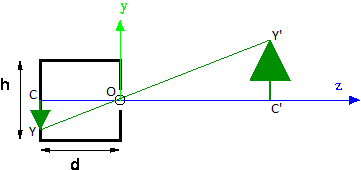
\includegraphics[width=280pt]{imgs/pinhole-and-tree2.png}
	\caption{Esempio cattura immagine con sensore pinhole.}
	\label{vis:stereo:pinhole}
\end{figure} 
Nel modello teorico in esame e con riferimento all'immagine \ref{vis:stereo:pinhole}, si considera una camera chiusa con un foro puntiforme (in pratica molto piccolo). La scatola è caratterizzata da due grandezze $d$ ed $h$. La prima è detta \textbf{distanza focale} è come si vedrà la sua conoscenza risulterà fondamentale nei ragionamenti che seguono. La seconda rappresenta grandezza la grandezza del film o pellicola o in chiave moderna la dimensione del sensore CMOS. Si fa notare che la scelta di quest'ultime grandezze definisce \textbf{l'angolo di visione} della camera, cioè il massimo angolo di ingresso dei raggi che possono essere catturati. Ad esempio, se si tiene fissata la grandezza del film e si diminuisce la distanza focale, si sarà in grado di catturare una porzione del mondo più ampia. In effetti sensori di questo tipo sono detti panoramici.
Se si considera un raggio di luce riflesso da un oggetto, ad esempio quello riflesso dalla punta dell'albero in figura, quest'ultimo "entrerà" attraverso il foro nella camera scura e verrà proiettato sulla pellicola o il sensore. Sempre dalla stessa immagine si può notare un importate aspetto geometrico, cioè che i triangoli $\widehat{COY}$ e $\widehat{C^{'}OY^{'}}$ sono simili.

Il precedente modello risulta per ovvie ragioni molto semplificato. In un sensore reale si possono considerare un numero molto maggiore di parametri e fattori. Ad esempio non si può far a meno di citare che le camere reali sono dotate di \textbf{lenti} atte a emulare il funzionamento del pinhole. Queste lenti introducono un inevitabile \textbf{distorsione} che fa si che un pixel dell'immagine non rappresenti il raggio di luce corretto. Questo fa venire meno la precedente proprietà per cui i suddetti triangoli sono simili. Fortunatamente tale distorsione può essere eliminata (quasi del tutto) attraverso procedure di calibrazione e raddrizzamento. In \cite{bib5} è indicato in dettaglio il funzionamento di queste ultime. Brevemente, le coordinate vengono ricalcolate utilizzando un modello della distorsione in forma di Taylor (tipicamente al sesto ordine) e ne vengono stimati i coefficienti attraverso una procedura sperimentale. In quest'ultima si fa catturare dal sensore un certo numero di immagini contenti un pattern noto (tipicamente una scacchiera o un insieme di cerchi) in posizioni differenti, poi i parametri vengono scelti con strumenti di minimizzazione.

Nel seguito di questa trattazione, non si farà più riferimento al fenomeno della distorsione, perché come già accennato può essere eliminato facilmente, complica la trattazione e risulta ben documentato in qualsiasi testo di visione artificiale ed online. 

Il modello Pinhole presenta però un inconveniente, cioè l'immagine catturata risulta capovolta. In effetti, il problema sorge dal fatto che il modello in questione cerca di mimare il funzionamento fisico del sensore, ma a livello matematico questo sforzo è inutile e può essere semplificato (in pratica i sensori reali provvedono a capovolgere l'immagine una volta catturata).
Si può utilizzare un modello del tutto equivalente detto \textbf{modello sintetico} o \text{virtuale}, mostrato in figura \ref{vis:stereo:virtuale}.
\begin{figure}[h!]
	\centering
	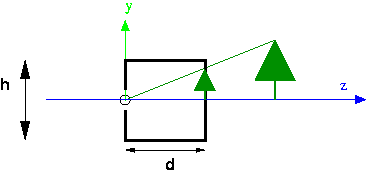
\includegraphics[width=280pt]{imgs/synthetic-and-tree.png}
	\caption{Esempio cattura immagine con sensore sintetico.}
	\label{vis:stereo:virtuale}
\end{figure} 
Il piano di cattura viene capovolto rispetto all'asse $y$, mentre le grandezze $h$ e $d$ hanno il medesimo significato. Il vantaggio di questa formulazione è che l'immagine catturata risulta orientata in modo corretto, lo svantaggio è che si è tralasciato il funzionamento fisico del sensore. Nel seguito verrà utilizzato quest'ultimo modello.

\subsection{Ricostruzione 3D}
\label{sec:stereo:ric3d}
Nel precedente paragrafo si è esplicato, seppur in modo teorico, il funzionamento del sensore fotografico. Si è potuto evincere che l'informazione raccolta dallo stesso altro non è che una \textbf{proiezione} su un piano (il piano dell'immagine) dei punti della scena. Pertanto, una parte dell'informazione è andata perduta e non può essere recuperata utilizzando un solo sensore. Risulta abbastanza intuitivo allora pensare di utilizzarne più di uno (almeno due) e cercare di combinare le informazioni ad essi relative.
\begin{figure}[h!]
	\centering
	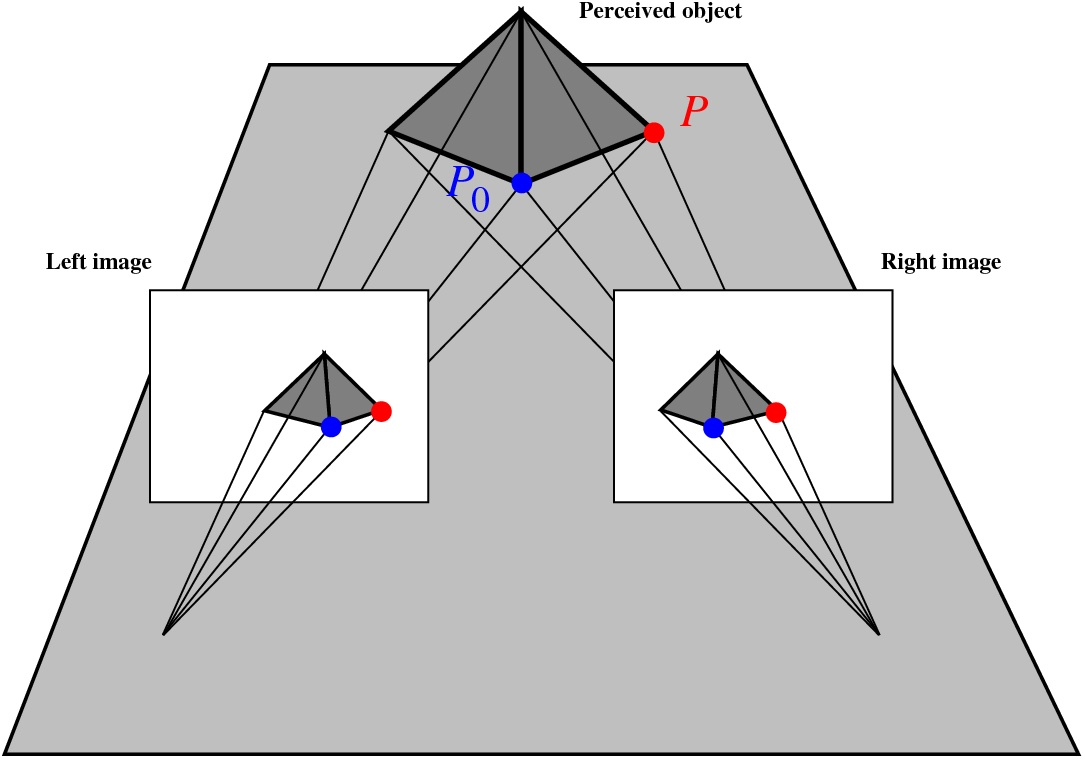
\includegraphics[width=420pt]{imgs/stereo2.jpg}
	\caption{Coppia di immagini catturate da due sensori differenti nella scena.}
	\label{vis:stereo:pair}
\end{figure} 
In generale, come già preannunciato, si possono utilizzare un numero arbitrario di sensori e possono essere posizionati in differenti maniere (purché catturino una parte comune della scena). Ad esempio in figura \ref{vis:stereo:pair} due immagini sono state catturate da due sensori posti in una differente posizione. Si può evincere che le immagini risultanti sono diverse, ed in particolare le proiezioni dei punti $P$ e $P_0$ nella foto di destra risultano più spostati verso sinistra.

In questa sede si opta per una configurazione con due camere e \textbf{centro di fissazione} all'infinito, cioè il punto di intersezione degli assi di fissazione dei due sensori passanti per il punto di fuoco $O_i$ e il centro del piano dell'immagine $C_i$ è all'infinito; tali assi sono quindi paralleli. Si suppone inoltre che, rispetto ad un sistema di riferimento solidale al sensore di sinistra e con origine coincidente al punto $O_l$, il sensore di destra (e quindi il punto $O_r$) ha la sola coordinata X non nulla.
\begin{figure}[h!]
	\centering
	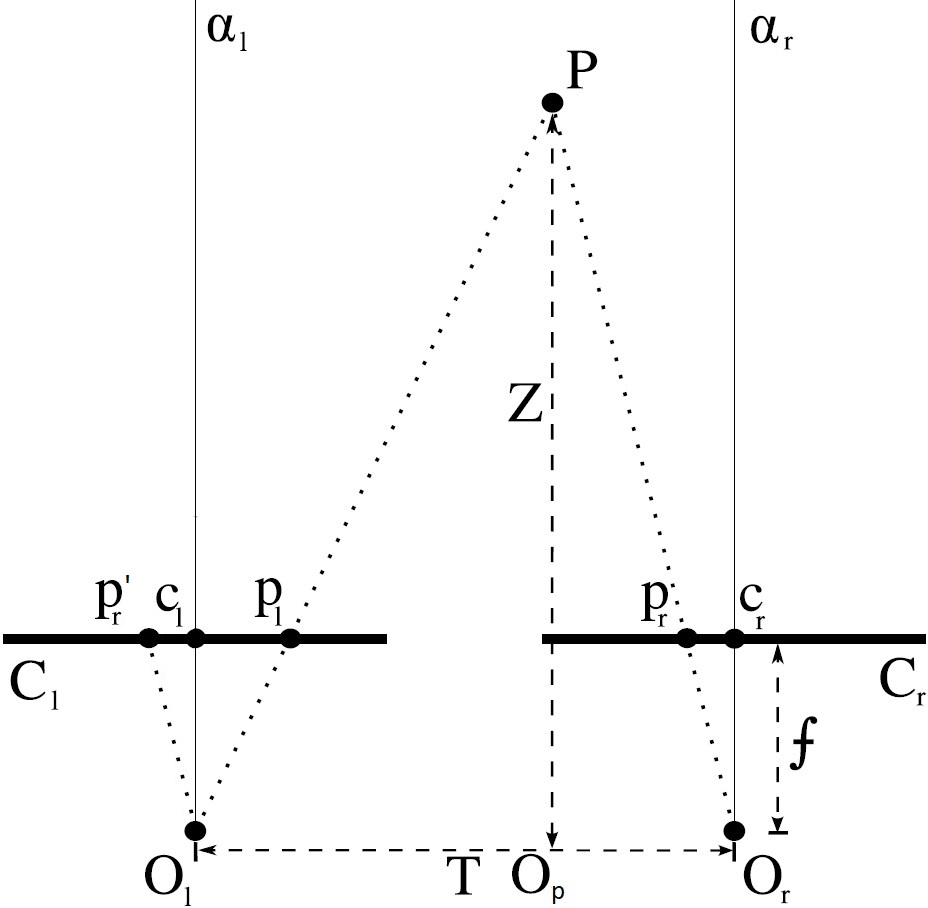
\includegraphics[width=360pt]{imgs/stereo.jpg}
	\caption{Configurazione sistema stereoscopico.}
	\label{vis:stereo:sistem}
\end{figure} 

Con riferimento alla figura \ref{vis:stereo:sistem}, si consideri un punto $P$ della scena, siano note la distanza tra i due sensori $T$, la lunghezza focale $f$ e i punti centrali delle camere $c_l$ e $c_r$ rispettivamente. Si suppone che il punto $P$ stesso venga catturato dalle due camere, cioè si conoscono i punti $p_l$ e $p_r$. \`{E} bene segnalare che l'individuazione di una corrispondenza tra due punti in due differenti immagini, e la comprensione quindi che essi corrispondano ad uno stesso punto della scena, è del tutto che banale. Allo state dell'arte attuale, esistono diversi approcci euristici caratterizzati alcuni da una miglior margine di errore, altri da un ridotto carico computazionale. Nel seguito si fornirà una soluzione a quest'ultimo problema.

Ragionando per via geometrica, si possono ottenere le coordinate geometriche cercate. Sempre dalla suddetta figura si può facilmente comprendere che i triangoli  $\widehat{C_lO_lp_l}$ e $\widehat{O_pPO_l}$ sono simili ed allo stesso modo $\widehat{C_rO_rp_r}$ e $\widehat{O_pPO_r}$ anch'essi lo sono. 

In primo luogo conviene calcolare un importante quantità, la disparità tra i punti $p_l$ e $p_r$. Essa è pari alla differenza in pixel delle coordinate x  tra i due suddetti punti nelle rispettive immagini. Si ribadisce che i due punti hanno la stessa coordinata y nelle immagini per via della struttura ipotizzata.
\begin{equation}
	d := p_{l_x} - p_{r_x}, d \ge 0, d \in \mathbb{Z}
\end{equation}

Se si immagina di "spostare" il triangolo $\widehat{C_rO_rp_r}$ tale da far coincidere il segmento $\overline{C_rO_r}$ con $\overline{C_lO_l}$, il triangolo risultante $\widehat{p_r^{'}O_lp_l}$ è simile al triangolo $\widehat{O_lPO_r}$. Allora, si può calcolare la coordinata Z con la seguente proporzione.
\begin{equation}
Z := \frac{Tf}{d}
\end{equation}

Si fissa il sistema di riferimento dell'osservatore su $O_l$ e con riferimento sempre alla suddetta figura si pongono l'asse Z e X appartenenti al piano del foglio, orientati rispettivamente verso l'alto e verso destra. L'asse Y sarà uscente dal foglio a completare un sistema di riferimento destrorso. 
Per il calcolo della coordinata X si può ragionare nel seguente modo: dato che i triangoli $\widehat{p_r^{'}O_lp_l}$ è simile al triangolo $\widehat{O_lPO_r}$ allora il rapporto tra il segmento $\overline{p_lc_l}$ e la base del triangolo (la disparità) $p_l - p_r^{'} = d$ deve essere lo stesso che tra il segmento $\overline{O_lO_p} = X$ ed $\overline{O_lO_r} = T$. Ne segue che:
\begin{equation}
	X := \frac{(p_{l_x} - c_l) T}{d}
\end{equation}
Per la coordinata Y si può procedere in maniera analoga.

Si riportano infine per comodità le relazioni individuate:
\begin{align}
	d &:= p_{l_x} - p_{r_x}, d \ge 0, d \in \mathbb{Z},\\
	X &:= \frac{(p_{l_x} - c_{l_x}) T}{d},\\
	Y &:= \frac{(p_{l_y} - c_{l_y}) T}{d},\\
	Z &:= \frac{Tf}{d}
\end{align}

Al fine di completare il discorso intrapreso conviene dare una risposta al problema su posto. Si è infatti sollevato il problema relativo al "riconoscimento" dei punti $p_l$ e $p_r$. Si è già accennato inoltre che esistono molteplici soluzioni a questo problema, ognuna con le sue particolarità. Ad esempio si può citare lo stereo block matcher (stereoBM), il quale esegue un confronto fra blocchi di immagini al fine di individuare lo stesso blocco nelle due immagini stereo. Esso utilizza, al fine di efficienza, una delle osservazioni su fatte, cioè che (se le immagini non sono distorte) la coppia di punti $p_l$ e $p_r$ hanno la stessa coordinata Y nelle due immagini. Esegue quindi una ricerca in linea per tutti i punti dell'immagine di sinistra su quella di destra.

In questa sede, siccome non ci si pone il problema di ottenere un informazione spaziale per tutti i punti della scena ma ne basta un sottoinsieme, si propone l'utilizzo del seguente metodo. Si può infatti ricorrere allo strumento introdotto nel paragrafo precedente: il \textbf{Feature Detection}. 

Tale strumento può essere utilizzato nella seguente maniera: \textit{un punto chiave è un oggetto che può essere definito spostamento-invariante. Ad esempio infatti, uno spigolo resta uno spigolo anche se nell'immagine risulta traslato e/o ruotato (e scalato). Si possono allora ricercare i punti chiave nelle due immagini stereo (eventualmente in parallelo), confrontare i punti chiave trovati e individuare quindi, ove possibile, la relazione tra i punti chiave dell'immagine di sinistra e quella di destra. Trovate tali relazioni, per ogni coppia, si procede a calcolare la disparità e quindi alla ricostruzione dell'informazione spaziale come su visto.}


\section{Soluzione al problema}
\label{sec:vision:solution}
A questo punto della trattazione, si è in grado quindi di affermare che il problema \ref{prob:vis:gensets} ha soluzione e se ne può fornirne una che, come tra poco si vedrà, utilizza ancora il fondamentale strumento del Feature Detection. Si riporta di seguito la procedura sintetizzata, dove si indicano con $M_{sx}^0$ e $M_{dx}^0$ rispettivamente l'immagine catturata dal sensore di sinistra e quello di destra all'istante precedente e, analogamente, con $M_{sx}^1$ e $M_{dx}^1$ quelle catturate all'istante attuale.

La procedura risulta cosi composta:
\begin{enumerate}
	\item Si individuano i punti chiave in tutte le immagini utilizzando l'algoritmo FAST:
	\begin{equation}
		\nonumber [kp_{sx}^0, \; kp_{dx}^0, \; kp_{sx}^1, \; kp_{dx}^1] = trovaPuntiChiaveIn(M_{sx}^0, M_{dx}^0, M_{sx}^1, M_{dx}^1)
	\end{equation} 
	\item Si procede alla descrizione dei punti chiave utilizzando l'algoritmo BRIEF:
	\begin{equation}
		\nonumber [dp_{sx}^0, \; dp_{dx}^0, \; dp_{sx}^1, \; dp_{dx}^1] = descriviPuntiChiave(kp_{sx}^0, kp_{dx}^0, kp_{sx}^1, kp_{dx}^1)
	\end{equation}
	\item Si individuano le corrispondenze tra i descrittori nelle due immagini stereo, attraverso il comparatore a forza bruta, al fine di calcolare la disparità dei punti chiave individuati e generarne le coordinate spaziali.
	\begin{align}
		\nonumber &mtch^0 = trovaCorrispondenzaTra(dp_{sx}^0, \; dp_{dx}^0)\\
		\nonumber &P^0 = calcolaCoordinateSpaziali(M_{sx}^0, M_{dx}^0, mtch^0)\\
		\nonumber &mtch^1 = trovaCorrispondenzaTra(dp_{sx}^1, dp_{dx}^1)\\
		\nonumber &P^1 = calcolaCoordinateSpaziali(M_{sx}^1, M_{dx}^1, mtch^1)
	\end{align}
	\item Si individuano le corrispondenze tra i punti chiave trovati rispettivamente nelle immagini sinistre all'istante precedente e quello attuale, e si utilizza questa informazione per generare due set contenenti le coordinate, rispetto al sistema solidale all'osservatore, dello stesso punto prima e dopo lo spostamento.
	\begin{align}
		\nonumber &mtch^{01} = trovaCorrispondenzaTra(dp_{sx}^0, dp_{sx}^1)\\
		\nonumber &[S^0, S^1] = generaSet(P^0, P^1, mtch^{01})
	\end{align}
\end{enumerate}

Si conclude infine sottolineando che nella precedente procedura diverse ottimizzazioni possono essere effettuate, e sono state effettuate. Si è scelto di riportarla in questa forma per maggiore chiarezza. Infatti, si può:
\begin{enumerate}
	\item mantenere i punti chiave e le rispettive descrizioni al fine di utilizzarle al passo successivo.
	\item le ricerche dei punti chiave nelle diverse immagini possono essere fatte in parallelo e così anche per il calcolo dei descrittori.
	\item il calcolo delle coordinate spaziali dei punti chiave può essere evitato per i punti per i quali non si è riuscito a trovare una corrispondenza prima e dopo lo spostamento.
\end{enumerate}



%mettere algoritmo finale che usa i due capitoli prima

